\documentclass[3p]{elsarticle}
\usepackage{ae,aecompl}
\usepackage[T1]{fontenc}
\usepackage[utf8]{inputenc}
\usepackage{pgfplots}
\usepackage{pst-plot}
\usepackage{tikz}
\usepgfplotslibrary{external}
\tikzexternalize
\usepackage{amsmath}
\usepackage{amssymb}
\usepackage{gensymb}
\usepackage{upgreek}
\usepackage{float}
\usepackage{indentfirst}
\parskip=0pt

\begin{document}

\begin{frontmatter}

\title{Potentiometric Scanning Electrochemical Microscopic Mapping of the Belousov-Zhabotinsky Oscillating Reaction}
\cortext[cor]{Corresponding author}
\author[akiss]{András Kiss\corref{cor}}
\address[akiss, gnagy]{Department of General and Physical Chemistry, Faculty of Sciences, University of Pécs, 7624 Pécs, Ifjúság útja 6, Hungary}
%\address[akiss, gnagy]{János Szentágothai Research Centre, University of Pécs, 7624 Pécs, Ifjúság Útja 20, Hungary}
\ead{akiss@gamma.ttk.pte.hu}
\author[gnagy]{Géza Nagy}
\ead{g-nagy@gamma.ttk.pte.hu}


\begin{abstract}

Patterns emerging in a distributed Belousov-Zhabotinsky reaction are usually studied with optical methods.
However, these methods provide only approximate information about the oxidation state of an indicator, and they cannot be applied when there is no indicator dye.
To gather additional information about the processes involved in the reaction, electrochemical methods can be used.
Using the appropriate electrodes, changes in bromide ion activity, pH and redox potential can be monitored.
Unfortunately, these methods will influence the studied system, since they require electrodes to be placed inside the reaction mixture.
This poses no problem when the studied reaction is stirred, but in a distributed system the electrodes -- depending on their size -- will influence the formation of spatial patterns, especially if one of them moves, for instance when used as a measuring tip in scanning electrochemical microscopy (SECM).

In this paper we show that, using a sufficiently small indicator electrode, these effects can be minimized to a point where no evidence of any disturbance to the reaction can be observed.
The first spatiotemporal SECM image about a distributed Belousov-Zhabotinsky reaction is shown, overlayed on top of the corresponding optical spatiotemporal image.
It was achieved by using a fine ($d_o = 7\, \upmu$m) carbon microelectrode with $\leq 1\, \upmu$m immersion depth.

\end{abstract}
\begin{keyword}
	Belousov-Zhabotinksy oscillating reaction \sep scanning electrochemical microscopy \sep potentiometry \sep microelectrode
\end{keyword}
\end{frontmatter}

\section{Introduction}

\section{Materials and methods}
\paragraph{The Belousov-Zhabotinsky reaction} 
%The initial concentrations of the reactants for the reaction is given in Table \ref{table:recipe}.
To start the reaction, the method that is described in \cite{winfree} was used.
Solution ''A,, was prepared by adding 2 ml of concentrated sulfuric acid and 5 g sodium bromate to 67 ml water.
Solution ,,B'' was 1 g malonic acid dissolved in 10 ml of water, solution ,,C'' was 1 g sodium bromate dissolved in 10 ml of water.
2 ml of ,,A'', 0.333 ml of ,,B'' and 0.166 ml ,,C'' was added to a small Petri dish ($d = 4 \,$cm).
After the yellow color of bromine vanished, 0.333 ml of 25 mM phenantroline ferrous sulfate was added, and the reaction mixture was stirred by a glass rod for a few seconds.
At this stage, the spontaneous formation of spatial patterns started.

\paragraph{Scanning Electrochemical Microscopy} A double wall Ag/AgCl/3 M KCl/0.1 M CH$_3$COOLi reference electrode was placed inside the reaction mixture, close to the edge of the Petri dish.
Then, a $d_o = 7\, \upmu$m carbon microelectrode was submersed $\leq$ 1 $\upmu$m into the reaction.
To accomplish it, the tip of the microelectrode was brought to contact with the reaction mixture by approaching the surface in 100 $\upmu$m increments using the Z axis of the SECM.
During this step, the potential of the microelectrode was continuously monitored.
When a sudden jump in the potential was observed -- as a consequence of the microelectrode making contact with the reaction mixture --, the microelectrode was retracted by 100 $\upmu$m.
Then, it was approached to the surface with increments of 1 $\upmu$m until it made contact with the surface again.
After the initial positioning, the scanning was started on a 10 mm long scanline with 200 $\upmu$m step size and 2000 $\upmu$m/s translation speed.
0.1 s was spent moving between adjacent data acqusition points, and 0.4 s was allowed for the potentiometric cell at every point to reach equilibrium potential to reduce potentiometric lag.
Scanning and recording was performed in both directions.
Altogether 6 back and forth cycles were performed.

\paragraph{Carbon microelectrode} The carbon microelectrode was prepared using a $d_o = 7\, \upmu$m carbon fiber that was isolated from a Toray Torayca T700S 24K tow (19002 50th Avenue East, Tacoma, WA 98446).
A single $\approx$ 1 cm long fiber was soldered into the hole of a round female pin header that was purchased from a local electronics store. 
The other end of the header was soldered to a d = 1 mm isolated copper wire to provide electrical connectivity and mechanical strength. 

\paragraph{Optical obseravtion}
The reaction was filmed with the camera of a Nexus 5 cell phone in 4k resolution.
The space-time plot was prepared using Blender 2.78 software by grabbing linear, 1 pixel high images from every 30th frame of the video (1 s interval).
The image sequence was assambled by stacking the grabs vertically using Imagemagick 1.3.20.
The overlayed optical-electrochemical plot was created by Gnuplot 4.6.6.

\begin{table}
                \caption{Initial concentrations of the reactants for the reaction.}
                \label{table:recipe}
                \centering
                \begin{tabular}{r c}
                        Reactant & Concentration \\
                        \hline
                        1 & 2 \\
                \end{tabular}
\end{table}


\section{Results and discussion}

\def\s{0.5}
\begin{figure}
\centering
% trim = top left bottom right
\includegraphics[trim = 10mm 20mm 0mm 10mm, clip, width=\s\textwidth, angle=-90]{spacetime.eps}
\caption{}
\label{fig:2d}
\end{figure}

%\begin{figure}
%\centering
%% trim = top left bottom right
%\includegraphics[trim = 10mm 20mm 0mm 10mm, clip, width=\s\textwidth]{microelectrode.jpg}
%\caption{}
%\label{fig:2d}
%\end{figure}

\def\s{0.15}
\def\left{70}
\def\bottom{120}
\def\right{50}
\def\top{30}
\begin{figure}
\centering
\begin{tikzpicture}
    \draw (0, 0) node[inner sep=0] {\includegraphics[trim = \left mm \bottom mm \right mm \top mm, clip, width=\s\textwidth]{0.png}};
    \draw (3.8, 1) node {a};
\end{tikzpicture}
\begin{tikzpicture}
    \draw (0, 0) node[inner sep=0] {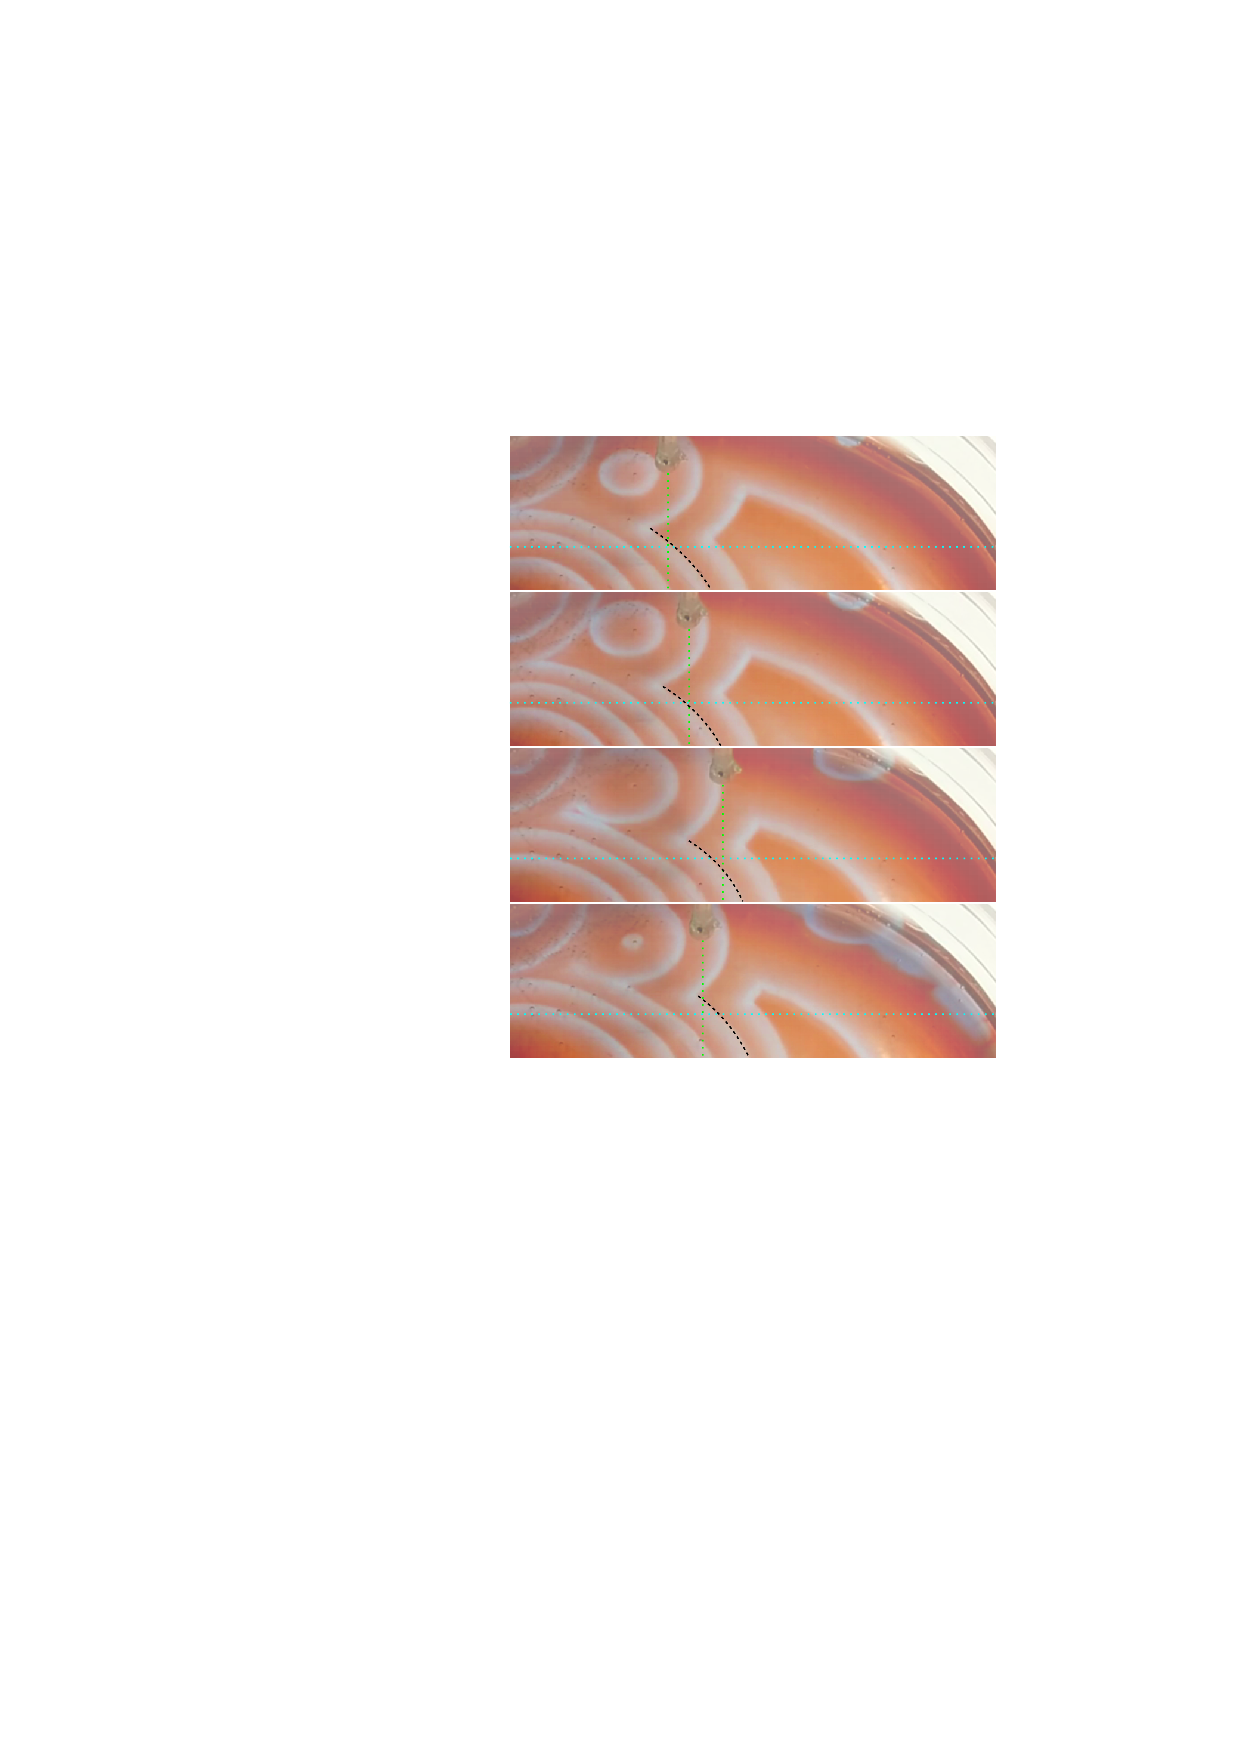
\includegraphics[trim = \left mm \bottom mm \right mm \top mm, clip, width=\s\textwidth]{1.png}};
    \draw (3.8, 1) node {b};
\end{tikzpicture}
\begin{tikzpicture}
    \draw (0, 0) node[inner sep=0] {\includegraphics[trim = \left mm \bottom mm \right mm \top mm, clip, width=\s\textwidth]{2.png}};
    \draw (3.8, 1) node {c};
\end{tikzpicture}
\begin{tikzpicture}
    \draw (0, 0) node[inner sep=0] {\includegraphics[trim = \left mm \bottom mm \right mm \top mm, clip, width=\s\textwidth]{3.png}};
    \draw (3.8, 1) node {d};
\end{tikzpicture}
\caption{}
\label{fig:2d}
\end{figure}

%\begin{tikzpicture}
%  \begin{axis}
%    \addplot3[colormap/viridis, surf, very thick] table {17101308_st_lines.txt};
%    %\addplot3[color=black, surf, very thick] table {17101308_st_lines.txt};
%  \end{axis}
%\end{tikzpicture}


\section{Conclusions}

\section*{References}

\begin{thebibliography}{5}
\bibitem{winfree} Winfree, Arthur T. The geometry of biological time. Vol. 12. Springer Science \& Business Media, 2001.

\end{thebibliography}


\end{document}
